%%
% Please see https://bitbucket.org/rivanvx/beamer/wiki/Home for obtaining beamer.
%%
\documentclass{beamer}

\usetheme{Luebeck}
\usecolortheme{crane}
\setbeamertemplate{section in toc}[ball unnumbered]
\setbeamertemplate{subsection in toc}[ball unnumbered]

\usepackage[T1]{fontenc}
\usepackage{beramono}
\usepackage{graphicx}
\usepackage{hyperref}
\usepackage{pifont}
\usepackage{listings}
\usepackage{xcolor}
\usepackage{multicol}


%\definecolor{darkgreen}{rgb}{0.,0.6,0.}

\newcounter{questionizeIndex}

\newenvironment{questionize}[1][0]{%
    \setbeamercovered{invisible}%
    \setcounter{questionizeIndex}{#1}%
    \begin{itemize}%
}{ %
    \end{itemize}%
}

\newcommand{\question}[2]{%
    % #1: question
    % #2: answer (replaces question)
    \stepcounter{questionizeIndex}%
    \item<\value{questionizeIndex}->%
    \only<\value{questionizeIndex}>{#1}%
    \stepcounter{questionizeIndex}%
    \only<\value{questionizeIndex}->{#2}%
}

\newcommand{\lquestion}[4]{%
    % #1: question label
    % #2: question
    % #3: answer label
    % #4: answer (replaces question)
    \stepcounter{questionizeIndex}%
    \item[\only<\value{questionizeIndex}->{\alt<\value{questionizeIndex}>{#1}{#3}}]<\value{questionizeIndex}->%
    \only<\value{questionizeIndex}>{#2}%
    \stepcounter{questionizeIndex}%
    \only<\value{questionizeIndex}->{#4}%
}

\newcommand{\cquestion}[2]{\question{#2}{\color{#1}{#2}}}

\newcommand{\ctrue}[1]{\cquestion{darkgreen}{#1}}
\newcommand{\cfalse}[1]{\cquestion{red}{#1}}

\newcommand{\ltrue}[1]{\lquestion{\textbf{?}}{#1}{$\checkmark$}{#1}}
\newcommand{\lfalse}[1]{\lquestion{\textbf{?}}{#1}{$\times$}{#1}}

\lstset{
    basicstyle=\footnotesize\ttfamily,
    breaklines=true
}


\hypersetup{%
  colorlinks=true,% hyperlinks will be black
  pdfborderstyle={/S/U/W 1}% border style will be underline of width 1pt
}
\begin{document}

\title{MSiA490 SEC20/28\\ Text Analytics}
\subtitle{Lab 1 - Tokenization and Beyond}
\author{Timo Wang}
\institute{Northwestern University}
\date{September 17, 2020}

\begin{frame}
    \titlepage
\end{frame}

\begin{frame}{Overview}
    \tableofcontents[hideallsubsections]
\end{frame}

\section{Who is Timo?}
\begin{frame}
    \frametitle{Who is Timo?}
    \begin{itemize}
        \item Third-year PhD student in Computer Science
        \item Academic experience
        \begin{itemize}
            \item Unsupervised multi-Document summarization
            \item Knowledge graph completion through inference
            \item Integrated frontend interface for AI systems
        \end{itemize}
        \item Industry experience
        \begin{itemize}
            \item Front-end developer
        \end{itemize}
    \end{itemize}
\end{frame}

%\section{What is tokenization?}
%\subsection{Raw text}
%\begin{frame}
%    \frametitle{What is tokenization?}
%    \framesubtitle{Raw text}
%    \begin{figure}
%        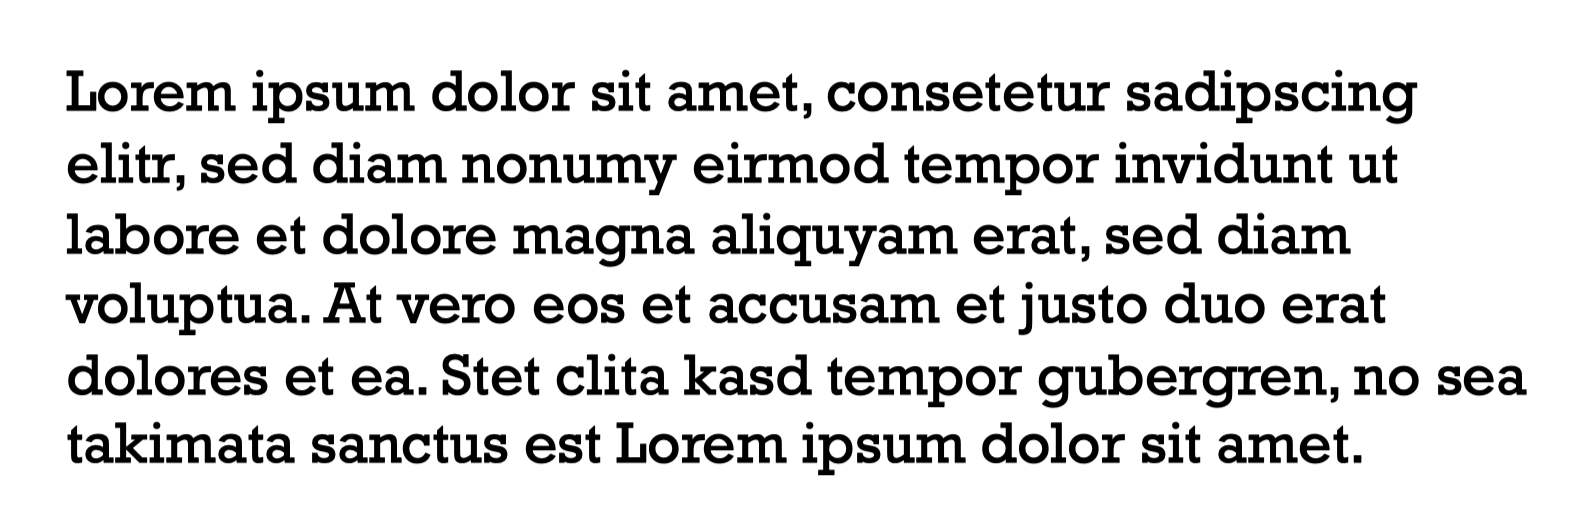
\includegraphics[scale=0.3]{raw-text}    
%    \end{figure}
%\end{frame}
%
%\subsection{Sentence-level tokenization}
%\begin{frame}
%    \frametitle{What is tokenization?}
%    \framesubtitle{Sentence-level tokenization}
%    \begin{figure}
%        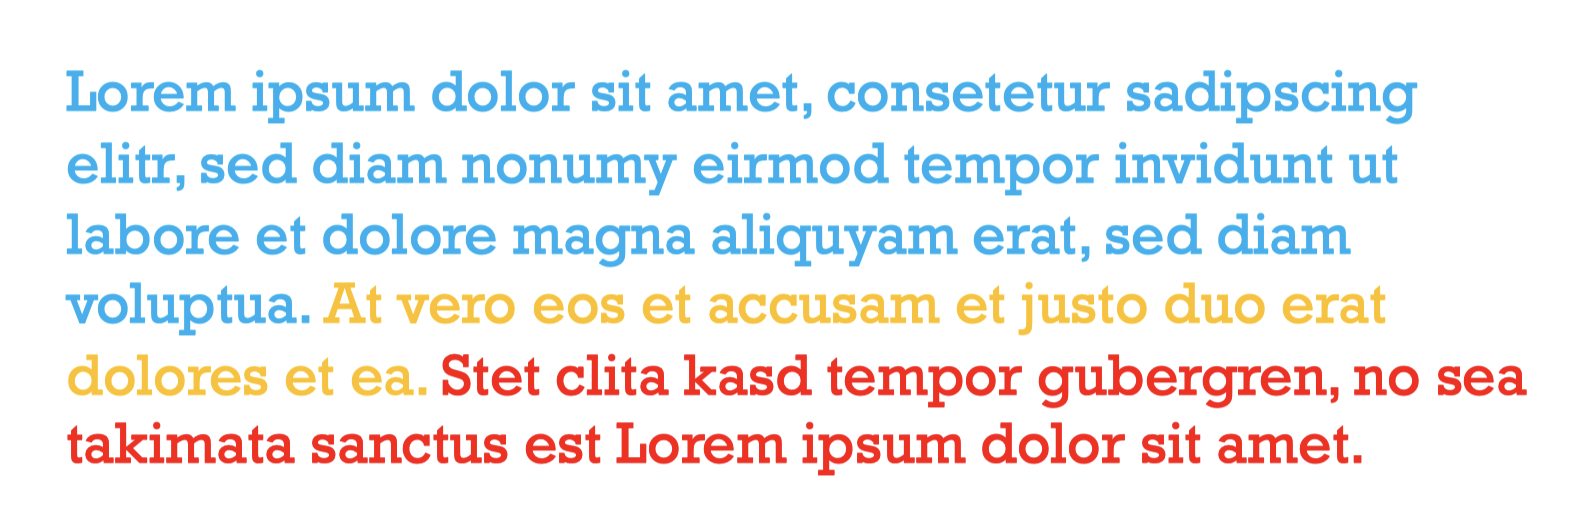
\includegraphics[scale=0.3]{sent}  
%    \end{figure}
%\end{frame}
%
%\subsection{Word-level tokenization}
%\begin{frame}
%    \frametitle{What is tokenization?}
%    \framesubtitle{Word-level tokenization}
%    \begin{figure}
%        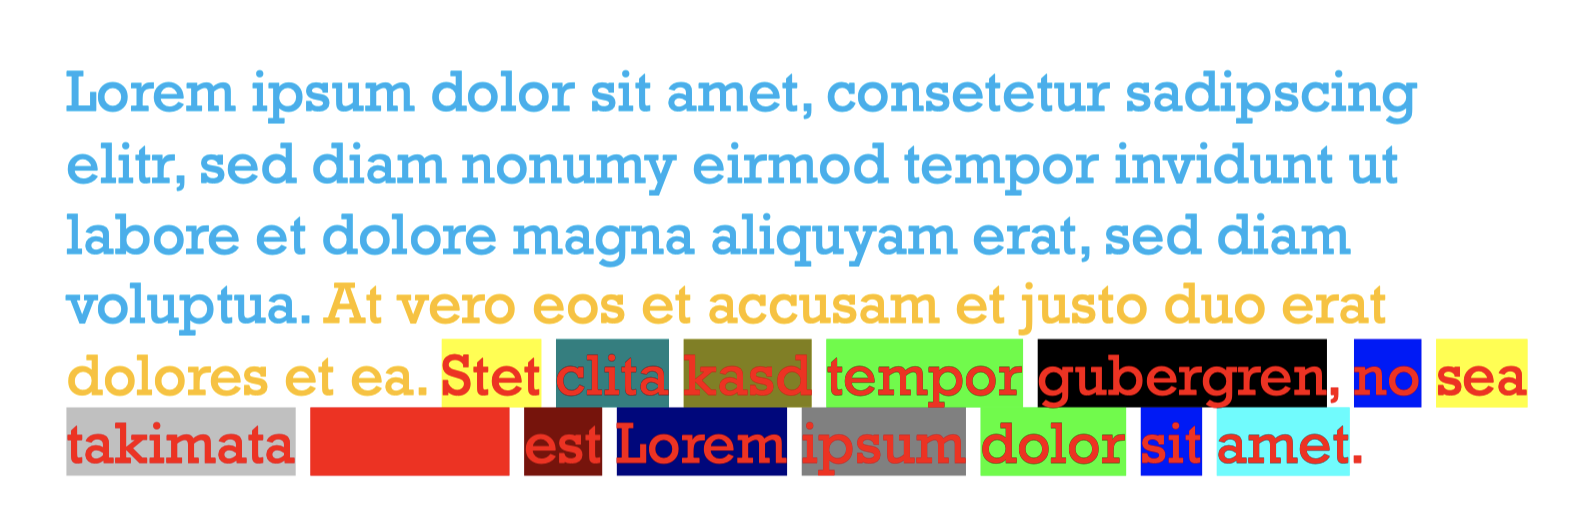
\includegraphics[scale=0.3]{word}    
%    \end{figure}
%\end{frame}

\section{Tokenization with common libraries}
\begin{frame}
    \frametitle{Tokenization with common libraries}
    \framesubtitle{Overview}
    \begin{itemize}
        \item NLTK
        \item Spacy
        \item Stanford Stanza
    \end{itemize}
\end{frame}

\subsection{NLTK}
\begin{frame}[containsverbatim]
    \frametitle{Tokenization with common libraries}
    \framesubtitle{NLTK -- Installation}
    
    \begin{block}{Shell}
        \begin{lstlisting}
pip install nltk
        \end{lstlisting}
    \end{block}
    \begin{block}{Python Console}
        \begin{lstlisting}
import nltk
nltk.download()
        \end{lstlisting}
    \end{block}
    
\end{frame}

\begin{frame}[containsverbatim]
    \frametitle{Tokenization with common libraries}
    \framesubtitle{NLTK -- Sentence-level}
    \begin{block}{Python Console}
        \begin{lstlisting}
from nltk.tokenize import sent_tokenize

text = `I am happy. I am sleepy. I am dreamy.'
sents = sent_tokenize(text)
        \end{lstlisting}    
    \end{block}

\end{frame}

\begin{frame}[containsverbatim]
    \frametitle{Tokenization with common libraries}
    \framesubtitle{NLTK -- Word-level}
    \begin{block}{Python Console}
        \begin{lstlisting}
from nltk.tokenize import word_tokenize

text = `I am happy. I am sleepy. I am dreamy.' 
words = word_tokenize(text)
        \end{lstlisting}    
    \end{block}

\end{frame}

\subsection{Spacy}
\begin{frame}[containsverbatim]
    \frametitle{Tokenization with common libraries}
    \framesubtitle{Spacy -- Installation}
    \begin{block}{Shell}
        \begin{lstlisting}
pip install spacy
python -m spacy download en_core_web_sm
        \end{lstlisting}    
    \end{block}

\end{frame}

\begin{frame}[containsverbatim]
    \frametitle{Tokenization with common libraries}
    \framesubtitle{Spacy -- Sentence-level}
    \begin{block}{Python Console}
        \begin{lstlisting}
import spacy

nlp = spacy.load('en_core_web_sm')
nlp.add_pipe(nlp.create_pipe('sentencizer'))

text = `I am happy. I am sleepy. I am dreamy.' 
doc = nlp(text)

sents = [sent.string.strip() for sent in doc.sents]        
        \end{lstlisting}        
    \end{block}

\end{frame}

\begin{frame}[containsverbatim]
    \frametitle{Tokenization with common libraries}
    \framesubtitle{Spacy -- Word-level}
    \begin{block}{Python Console}
        \begin{lstlisting}
import spacy

nlp = spacy.load('en_core_web_sm')
nlp.add_pipe(nlp.create_pipe('sentencizer'))

text = `I am happy. I am sleepy. I am dreamy.' 
doc = nlp(text)

words = [token.text for token in doc]
        \end{lstlisting}    
    \end{block}

\end{frame}


\subsection{Stanford Stanza}
\begin{frame}[containsverbatim]
    \frametitle{Tokenization with common libraries}
    \framesubtitle{Stanford Stanza -- Installation}
    \begin{block}{Shell}
        \begin{lstlisting}
pip install stanza
        \end{lstlisting}    
    \end{block}
    
    \begin{block}{Python Console}
        \begin{lstlisting}
import stanza
stanza.download('en')
        \end{lstlisting}    
    \end{block}
\end{frame}

\begin{frame}[containsverbatim]
    \frametitle{Tokenization with common libraries}
    \framesubtitle{Stanford Stanza -- Sentence-level}
    \begin{block}{Python Console}
        \begin{lstlisting}
import stanza

text = `I am happy. I am sleepy. I am dreamy.'

nlp = stanza.Pipeline('en')
doc = nlp(text)
sents = [' '.join([token.text for token in sentence.tokens]).strip() for sentence in doc.sentences]
        \end{lstlisting}    
    \end{block}

\end{frame}

\begin{frame}[containsverbatim]
    \frametitle{Tokenization with common libraries}
    \framesubtitle{Stanford Stanza -- Word-level}
    \begin{block}{Python Console}
        \begin{lstlisting}
from functools import reduce

import stanza

text = `I am happy. I am sleepy. I am dreamy.'

nlp = stanza.Pipeline('en')
words_by_sentence = [[token.text for token in sentence.tokens] for sentence in doc.sentences]
words = reduce(lambda lst1,lst2: lst1 + lst2, words_by_sentence)

        \end{lstlisting}    
    \end{block}
\end{frame}

\subsection{Extra resources}
\begin{frame}
    \frametitle{Tokenization with common libraries}
    \framesubtitle{Extra resources}
    \begin{itemize}
        \item Miniconda: \href{https://docs.conda.io/en/latest/miniconda.html}{https://docs.conda.io/en/latest/miniconda.html}.
        \item NLTK: \href{https://www.nltk.org/}{https://www.nltk.org/}
        \item Spacy: \href{https://spacy.io/usage/spacy-101}{https://spacy.io/usage/spacy-101}
        \item Stanford Stanza: \href{https://stanfordnlp.github.io/stanza/}{https://stanfordnlp.github.io/stanza/}
    \end{itemize}
\end{frame}



\section{Hands on}
\begin{frame}
    \frametitle{Hands on}
    \framesubtitle{Tokenization, stemming and POS tagging}
    \begin{block}{Task}
        \begin{enumerate}
            \item Install and evaluate 2 to 3 text preprocessing libraries (in python or Java).
            \item Download a publicly available text corpus.
            \item Apply tokenization, stemming and POS tagging on the full corpus.
        \end{enumerate}
    \end{block}
    \begin{block}{Note}
        \scriptsize
        Keep an eye out for the time/memory consumption of each library as well as their ease of use.     
    \end{block}
\end{frame}

\section{Quiz}
\subsection{Task 1}
\begin{frame}
    \frametitle{Quiz}
    \framesubtitle{Task 1}
    Which library do you find easiest to use for tokenization?
    \begin{enumerate}
        \item[A] NLTK
        \item[B] Spacy
        \item[C] Stanford Stanza
        \item[D] Other
    \end{enumerate}
\end{frame}

\subsection{Task 2}
\begin{frame}
    \frametitle{Quiz}
    \framesubtitle{Task 2}
    Which library runs fastest for POS tagging?
    \begin{enumerate}
        \item[A] NLTK
        \item[B] Spacy
        \item[C] Stanford Stanza
        \item[D] Other
    \end{enumerate}
\end{frame}

\subsection{Task 3}
\begin{frame}
    \frametitle{Quiz}
    \framesubtitle{Task 3}
    Which library appears most memory efficient on your machine/OS of choice?
    \begin{enumerate}
        \item[A] NLTK
        \item[B] Spacy
        \item[C] Stanford Stanza
        \item[D] Other
    \end{enumerate}
\end{frame}

\section{Thoughts \& feedbacks}
\begin{frame}
    \frametitle{Thoughts \& feedbacks}
    \begin{itemize}
        \item Make slides available before each lab. 
    \end{itemize}
\end{frame}


\end{document}
